\chapter{graspologic} \label{chap:graspologic}

This chapter documents our first investigation into the alpha blocker treatment hypothesis in humans facing a severe respiratory illness. Importantly, this study leveraged large insurance claims databases and common health conditions during a period where the COVID-19 data environment was too immature to produce a sufficiently large and well-understood sample for this analysis. This chapter was originally published in Journal of Machine Learning Research in September 2019 (\burl{http://jmlr.org/papers/v20/19-490.html}) and is distributed under the terms of a Creative Commons Attribution License that permits unrestricted use and redistribution provided that the original author and source are credited.

%%%% MUST: add the citation for the chapter if it is a reprint or submitted paper
%% you can use enumerate or itemize environment if you have more than one paper 
%% \mybibexclude{} will exclude this citation from the final bibliography
%% if this paper appears somewhere else then remove \mybibexclude{} command

%%%% MUST: add the citation for the chapter if it is a reprint
% \begin{singlespace}         % you can also use onehalfspace to relax the spacing
%     This chapter is adapted from the following article with permission from ...
    
%     \fullcite{chung2019graspy}.
% \end{singlespace} 

\pagebreak

\section*{Abstract}
We introduce \graspy, a Python library devoted to statistical inference, machine learning, and visualization of random graphs and graph populations. This package  provides flexible and easy-to-use algorithms for analyzing and understanding graphs with a \sklearn compliant API. \graspy ~can be downloaded from Python Package Index (PyPi), and is released under the MIT open-source license. The documentation and all releases are available at \url{https://microsoft.github.io/graspologic/latest} and \url{https://github.com/microsoft/graspologic}, respectively.
\pagebreak


\section{Introduction}
Graphs, or networks, are a mathematical representation of data that consists of discrete objects (nodes or vertices) and relationships between these objects (edges). For example, if thinking of regions of a human brain as vertices, the edges can represent how strongly each pair of regions are connected to each other. 
Since graphs necessarily deal with relationships between nodes, many of the classical statistical assumptions about independence are violated. Thus, specific statistical methodology is required for performing robust statistical inference on graphs and populations of graphs \citep{survey-rdpg}. \graspy fills this gap by providing implementations of algorithms with strong statistical guarantees, such as graph and multi-graph embedding methods, two-graph hypothesis testing, and clustering of vertices of graphs. Many of the algorithms implemented in \graspy are flexible and can operate on graphs that are weighted or unweighted, as well as directed or undirected. All subsequent analysis in this thesis was performed using \graspy.

\section{Library Overview}
Overview of submodules available in \graspy is summarized in Figure \ref{fig:graspy}. The library contains functionality for fitting and sampling from random graph models, performing dimensionality reduction on graphs or populations of graphs (embedding), testing hypotheses on graphs, and plotting of graphs and embeddings.

The following provides brief overview of different submodules of \graspy, and more detailed overview and code usage can be found in the tutorial section of \graspy documentation at \url{https://microsoft.github.io/graspologic/latest/tutorials/index.html}.

\begin{figure}[t]
    \centering
    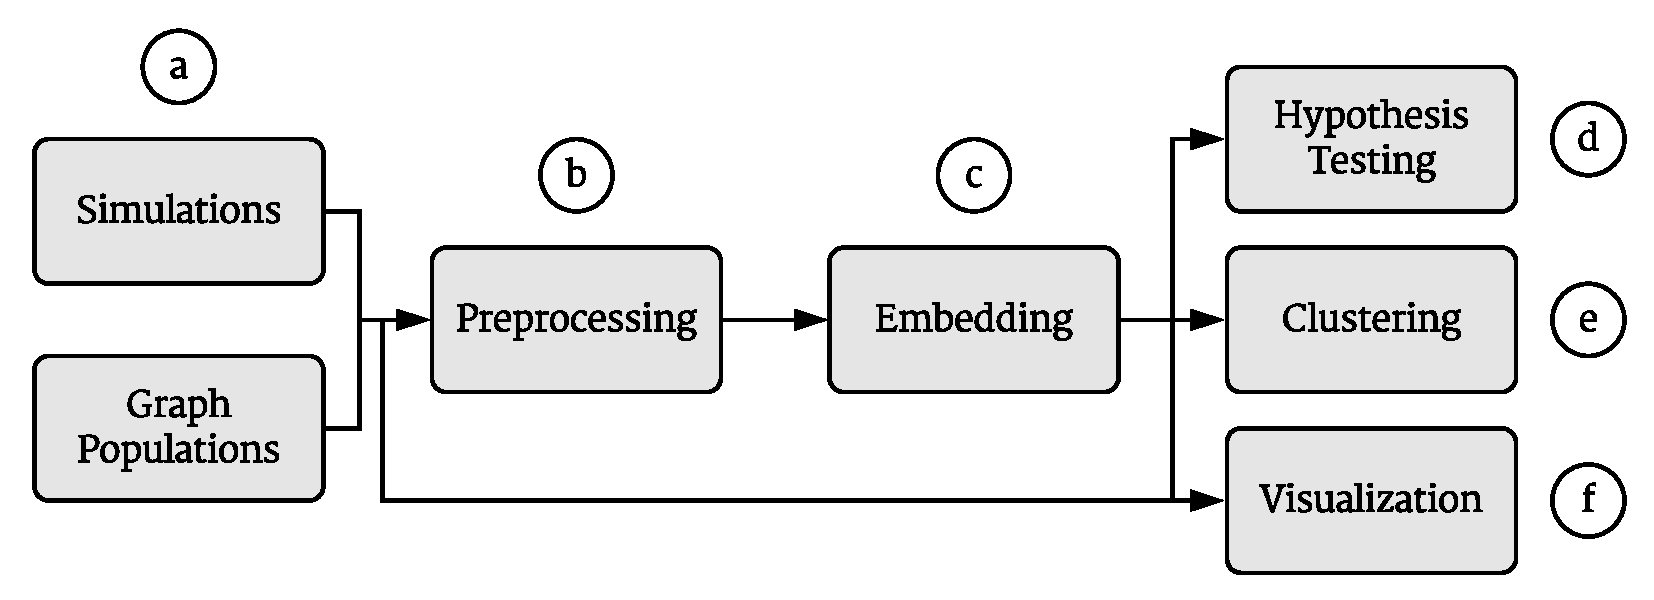
\includegraphics[width=.8\linewidth]{figures/graspy/graspy.pdf}
    \caption{Illustration of submodules and procedure for statistical inference on population of graphs. A detailed description of each submodule is given in section 2.}
    \label{fig:graspy}
\end{figure}

\subsection{Simulations (Figure \ref{fig:graspy}a)} Three classes of random graph models are implemented in \graspy: 1) Erd\H os-R\'enyi (ER) model, 2) stochastic block model (SBM), and 3) random dot product graph (RDPG) model. ER model is the simplest model, in which the model is parameterized by the number of vertices, $n$, and either $p$ that specifies a probability of an edge existing between a pair of vertices or $m$ that specifies the exact number of edges. All nodes have the same probability of connection to each other under the ER model. Unlike ER models, the SBM produces graphs containing communities, where vertices in each community share common probabilities of connection to every other community. The SBM is parameterized by the number of communities, $K$, a vector of probabilities of a node belonging to each community, $\tau$, and a probability matrix, $B\in[0,1]^{K \times K}$, that specifies the probability of edges within and between communities. An extension of the SBM, the Degree-corrected SBM (DCSBM) has an added parameter associated with each node that denotes its promiscuity in the graph, which is its relative degree among the other nodes in its community. Nodes still share the same relative probabilities of connection to each community, but the nodes within a community may have heterogeneous expected degrees. Finally, the RDPG model assumes that each vertex in the graph is associated with a latent vector in $\mathbb{R}^d$. The probability of an edge existing between pairs of vertices is determined by the dot product of the associated latent position vectors \citep{young2007random}. The RDPG is parameterized by an $n$ by $d$ matrix of these latent positions. \graspy provides implementations for sampling from each of these graph models given these parameters, as well as estimating the parameters of a model from a given graph. \graspy also allows for weighting functions and directed graphs when sampling from these models.

\subsection{Preprocessing (Figure \ref{fig:graspy}b)}
Various utility functions help the user input real data into \graspy or check simple attributes about a graph. Some examples include finding the largest connected component of a graph, finding the intersection or union of connected components across multiple graphs, transforming the weights of a graph, or checking whether a graph is directed. These functions speed the user's workflow when working with real data that may be messy or noisy before preprocessing.

\subsection{Embedding (Figure \ref{fig:graspy}c)}
Inference on random graphs depends on low-dimensional Euclidean representation of the vertices of graphs, known as \textit{latent positions}, typically given by spectral decompositions of adjacency or Laplacian matrices \citep{levin2017central}. Adjacency spectral embedding (ASE) and Laplacian spectral embedding (LSE) are methods for embedding a single graph, and omnibus embedding allows for embedding multiple graphs into the same dimensions such that the embeddings can be meaningfully compared. In addition, \graspy allows for the number of embedding dimensions to be automatically chosen by the algorithm of \cite{zhu2006automatic}. 

\begin{figure}[t!]
    \centering
    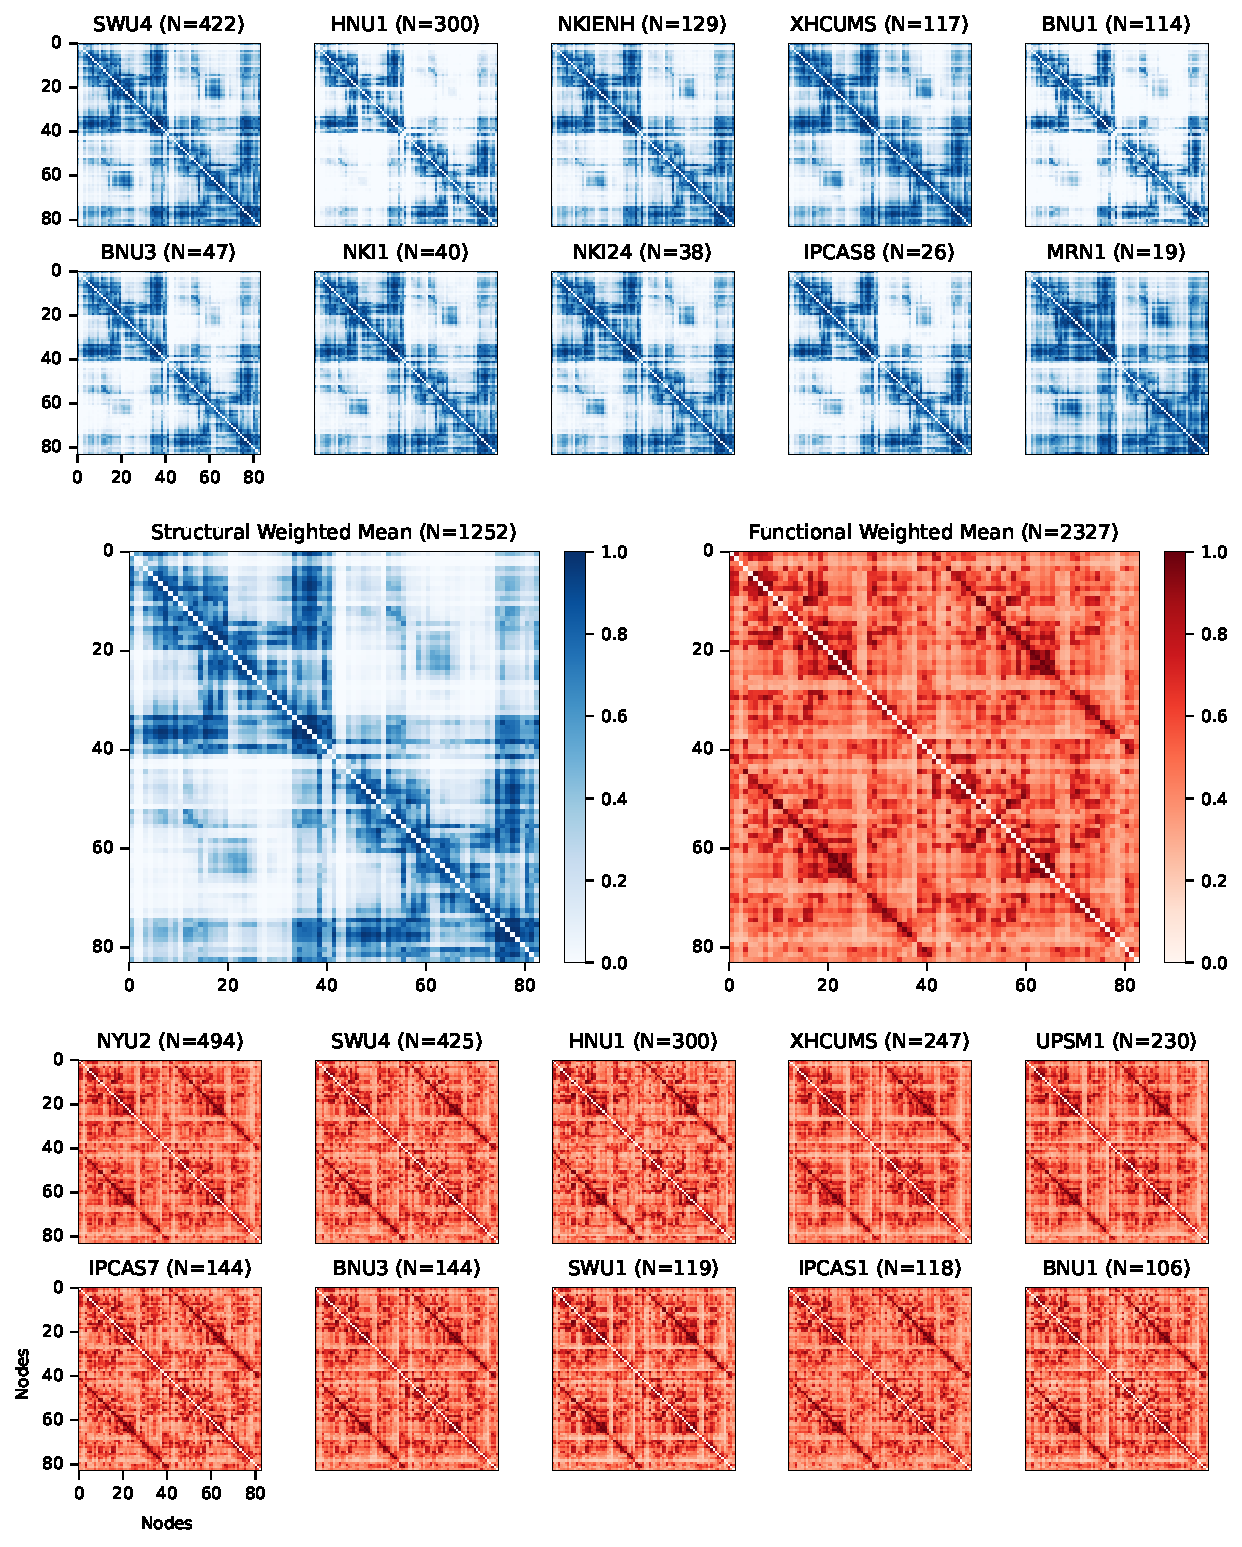
\includegraphics[width=1\textwidth]{figures/graspy/figure2.pdf}
    \caption{Connectome model fitting and complexity.  Larval Drosophila left mushroom body adjacency matrix (unweighted, directed), followed by random samples from four different statistical models of connectomes fit using \graspy: random dot product graph (RDPG), degree-corrected stochastic block model (DCSBM), stochastic block model (SBM), and Erd\H os-R\'enyi (ER). The bottom left shows the number of parameters for each, as compared to the 40,000+ number of parameters (possible edges) for the inhomogeneous Erd\H os-R\'enyi (IER) model in which all potential edges are specified. Blocks are sorted by size (number of member vertices) and nodes are sorted by degree within each block. The block labels correspond to K) Kenyon cells, P) projection neurons, O) mushroom body output neurons, I) mushroom body input neurons \citep{eichler2017complete}.
    }
    \label{fig:my_label}
\end{figure}

\subsection{Hypothesis Testing (Figure \ref{fig:graspy}d)}
Given two graphs, a natural question to ask is whether these graphs are both random samples from the same generative distribution. \graspy provides two types of test for this null hypothesis: semiparametric and nonparametric. Both tests are framed under the RDPG model, where the generative distribution can be modeled as a set of latent positions. The semiparametric test can only be performed on two graphs of the same size and with known correspondence between the vertices of the two graphs \citep{tang2017semiparametric}. Nonparametric testing can be performed on graphs without vertex alignment, or even with different numbers of vertices \citep{tang2014nonparametric}. Both tests provide a statistically principled way of claiming whether two observed graphs are the same; for example, one can test whether the brain connectivity graphs of siblings or twins came from the same generative distribution (Chung et al., in preparation). 

\subsection{Clustering (Figure \ref{fig:graspy}e)}
\graspy uses Gaussian mixture models (GMM) and k-means to compute the grouping structure of vertices after embedding. The number of clusters to fit for GMM is chosen by Bayesian information criterion (BIC), which is a penalized likelihood function to evaluate the quality of estimators. Similarly, the silhouette score is used to choose the number of clusters for k-means. Both functions sweep over a range of parameters and use the above metrics to choose clustering parameters in an unsupervised manner. 

\subsection{Plotting (Figure \ref{fig:graspy}f)}
\graspy extends \texttt{seaborn} to visualize graphs as adjacency matrices and embedded graphs as paired scatter plots \citep{seaborn}. Individual graphs can be visualized using \texttt{heatmap} function, and multiple graphs can be overlaid on top of each other using \texttt{gridplot} function. Both adjacency matrix visualizations can be sorted by various node metadata. \texttt{pairplot} can visualize high dimensional data, such as graphs in the embedded space, as a pairwise scatter plot.

\section{Conclusion}
\graspy is the first open-source Python package to perform robust statistical analysis on graphs and graph populations. Its compliance with the \sklearn API makes it an easy-to-use tool for anyone familiar with machine learning in Python. In addition, \graspy is implemented with an extensible class structure, making it easy to modify and add new algorithms to the package. As \graspy continues to grow and add functionality, we believe it will accelerate statistically-valid discovery in any field of study concerned with populations of graphs. 